\documentclass[onecolumn, draftclsnofoot,10pt, compsoc]{IEEEtran}
\usepackage{graphicx}
\usepackage{url}
\usepackage{setspace}
\usepackage{caption}
\graphicspath{ {/} }
\usepackage{geometry}
\usepackage{imakeidx}
\usepackage{float}
\makeindex[columns=1, options=-s lou3.ist]
\geometry{textheight=9.5in, textwidth=7in}

% 1. Fill in these details
\def \CapstoneTeamName{   The Visionaries}
\def \CapstoneTeamNumber{   3}
\def \GroupMemberOne{     Kien Tran}
\def \GroupMemberTwo{       Brian Wiltse}
\def \CapstoneProjectName{    Code3 Visionary}
\def \CapstoneSponsorCompany{ Levrum Data Technologies}
\def \CapstoneSponsorPerson{  Carl Niedner}

% 2. Uncomment the appropriate line below so that the document type works
\def \DocType{    
        %Requirements Document
        %Technology Review
        Design Document
        %Progress Report
        }
      
\newcommand{\NameSigPair}[1]{\par
\makebox[2.75in][r]{#1} \hfil   \makebox[3.25in]{\makebox[2.25in]{\hrulefill} \hfill    \makebox[.75in]{\hrulefill}}
\par\vspace{-12pt} \textit{\tiny\noindent
\makebox[2.75in]{} \hfil    \makebox[3.25in]{\makebox[2.25in][r]{Signature} \hfill  \makebox[.75in][r]{Date}}}}
% 3. If the document is not to be signed, uncomment the RENEWcommand below
%\renewcommand{\NameSigPair}[1]{#1}

%%%%%%%%%%%%%%%%%%%%%%%%%%%%%%%%%%%%%%%
\begin{document}

\begin{titlepage}
    \pagenumbering{gobble}
    \begin{singlespace}
      
\includegraphics[height=4cm]{coe_v_spot1}
        \hfill 
        % 4. If you have a logo, use this include graphics command to put it on the cover sheet.
        %\includegraphics[height=4cm]{CompanyLogo}   
        \par\vspace{.2in}
        \centering
        \scshape{
            \huge CS Capstone \DocType \par
            \large{Spring Term}\par
            {\large\today}\par
            \vspace{.5in}
            \textbf{\Huge\CapstoneProjectName}\par
            \vfill
            {\large Prepared for}\par
            \Huge \CapstoneSponsorCompany\par
            \vspace{5pt}
            {\Large\NameSigPair{\CapstoneSponsorPerson}\par}
            {\large Prepared by }\par
            Group\CapstoneTeamNumber\par
            % 5. comment out the line below this one if you do not wish to name your team
            %\CapstoneTeamName\par 
            \vspace{5pt}
            {\Large
                \NameSigPair{\GroupMemberOne}\par
                \NameSigPair{\GroupMemberTwo}\par
            }
            \vspace{20pt}
        }
        \begin{abstract}
                Emergency resources, such as fire stations, are expensive, long-term investments.
                Optimal placement of emergency resources involves considering the distribution of demand in a given jurisdiction.
                The Code3 Visionary project will utilize machine learning and statistical analysis to predict future distributions of emergency incidents in a given area, which will provide insight into the optimal placement of emergency resources. 
                This design document includes an overview and the scope of the Code3 Visionary project, as well as specifications for the Code3 Visionary application.
				The design views discussed are Code3 Visionary's data ingestion and feature extraction modules, application programming interface, machine learning and predictive model modules, and API.
        \end{abstract}
    \end{singlespace}
\end{titlepage}
\newpage
\pagenumbering{arabic}
\tableofcontents
% 7. uncomment this (if applicable). Consider adding a page break.
\newpage
\listoffigures
%\listoftables
\clearpage

% 8. now you write!
\section{Overview}
\begin{singlespace}
This design document describes the development of the Code3 Visionary (C3V) application. 
Brian Wiltse will be in charge of data ingestion and feature extraction. 
Kien Tran will manage the development of machine learning algorithms, creating a trained model, and the application programming interface. 
The Visionaries discuss the purpose of each component and how the components interact within C3V.
\begin{figure}[h!]
    \centering
    \includegraphics[height=10cm, width=17cm]{Code3VisionaryDiagram.eps}
    \caption{The design overview: Code3 Visionary}
    \label{fig:diagram}
\end{figure}
\subsection{Scope}
    This document describes plans for version 1.0 of the Code3 Visionary application, issued by Levrum Data Technologies.

    \subsection{Design Stakeholders}
        The following members of Levrum Data Technologies are stakeholders in Code3 Visionary:
        \begin{itemize}
            \item Ofer Heyman: President and CEO.
            \item Carl Niedner: VP of Product Development and Co-founder.
            \item Chester Ornes: VP of Engineering and Co-founder
        \end{itemize}

    \subsection{Context}
    Emergency services are a crucial part of a thriving community. When an individual calls 9-1-1, responders must arrive on the scene with minimal delay. A delay of minutes, or even seconds, can have deadly consequences. For this reason, police officers, firefighters, and emergency medical personnel constantly track emergency calls and the time it takes for responders to arrive on scene. Responders undergo training on procedures to reduce their response time when a call comes in. While procedures and well-trained personnel are critical elements of a timely emergency response, no amount of training can replace a lack of necessary resources.  
    
    Our project, Code3 Visionary (C3V), aims to provide command-level personnel with the information they need to ensure resources placed where they are most in-demand. 
    Using an area's demographics, zoning information, and prior emergency call logs, we will determine the factors that most highly correlate with various types of emergency calls.
    Based on our analysis, we aim to predict the number of each investigated call type that will occur in a given place at a future time, giving command-level personnel the information they need to plan ahead.
    At a high level, C3V involves building tools to prepare data for analysis, researching and implementing machine learning algorithms, and building an API that can display the results of our software's analysis. 
        
    Levrum Data Technologies' existing software, Code3 Strategist, allows users to perform what-if analyses for emergency resource allocation.
    In a what-if analyses, a user can run hypothetical emergency scenarios against custom resource allocation configurations.
    Code3 Visionary aims take this capability a step further and predict the need for emergency services in a given place and time.
    This would provide users with the most likely emergency scenarios, against which they can test their current or hypothetical resource allocations in Code3 Strategist \cite{TechReview}. 
    The scope of the current iteration of C3V is to assist Levrum with a proof of concept for their client in Charlotte, North Carolina.
    
    \subsection{Definitions}
    \begin{itemize}
        \item \textbf{areal interpolation:} Reaggregating data attributed to one shape to another shape. For example, reducing the population of a shape to be proportional to the remaining area after clipping the shape.
        \item \textbf{block group:} A subdivision of a U.S. tract for the U.S. Census.
        \textit{See also:} \textbf{tract}.
        \item \textbf{data ingestion:} The process of obtaining, transforming, and storing data for use in the feature extraction module. \textit{See also:} \textbf{feature extraction}.
        \item \textbf{feature extraction:} The process of obtaining useful values from data stored during the data ingestion process. \textit{See also:} \textbf{data ingestion}.
        \item \textbf{genetic algorithm:} Algorithm based off of natural selection to generate high quality solution to optimization and search problems. It uses methods such as mutation, crossover, and selection.
        \item \textbf{machine learning algorithm:} An algorithm that can learn from data and make predictions.
        \item \textbf{predictive model:} A model trained with machine-learning methods, used to make predictions.
        \textit{See also:} \textbf{machine learning algorithm}.
        \item \textbf{time} or \textbf{location of interest:} The time and area to which a predictive model applies. 
        \textit{See also:} \textbf{predictive model}.
        \item \textbf{tract:} A subdivision of a U.S. county for the U.S. Census.
        \item \textbf{traffic analysis zone (TAZ):} A subdivision of a U.S. county generally used for transportation planning. 

    \end{itemize}

    \subsection{Additional Information}
        \subsubsection{Changes}
        This document describes Code3 Visionary 1.0. The document was updated on February 23, 2018 with several modifications. Significant modifications to this document were planned and discussed with all interested parties before the first version was finalized. In general, the focus of their project has shifted from a standalone application to developing a proof of concept for predicting call volumes for a given time and location for Levrum's clients in Charlotte, NC.
        
        A further revision was made May 2, 2018. 
        As of this date, the scope of The Visionaries' contribution to the project is finalized and agreed upon 
        by Levrum and The Visionaries. 
        Design decisions, unknown at the time of the original document and prior revisions, are provided in detail.
        
        \subsubsection{Structure of the document}
        Section \ref{data_ingestion} describes how C3V will obtain and store data from various sources. 
        Section \ref{feature_extraction} describes how C3V will extract useful features from data stored during data ingestion. 
        Section \ref{application_interface} describes the application interface of C3V.
		Section \ref{machine_learning_algorithm} describes the machine learning algorithm C3V will use.
		Section \ref{trained_model} describes the predictive model that will be generated by C3V.
		Section \ref{api} describes the application programming interface that C3V will provide.

\section{Data Ingestion} \label{data_ingestion}
Data ingestion refers to the process of obtaining, manipulating, and storing raw data from various sources. 
Design concerns for the data ingestion process are:
\begin{itemize}
    \item \textbf{Testability.}\index{testing} The system shall be modular enough to allow testing for each major step of data collection: 
        \begin{itemize}
            \item Obtaining and appending Census data
            \item Appending incident counts
            \item Appending zoning data
            \item Areal interpolation
        \end{itemize}
    \item \textbf{Adaptability.} The system shall be able to generate a shapefile with U.S. Census demographics for an arbitrary county in the United States.  
    \item \textbf{Extensibilty and Modifiability.} The system shall use a pipeline structure, so that more data can be added to the final data set by creating a new data collection module and inserting it into the pipeline. 
\end{itemize}

    \subsection{Data Formats}
    Each data ingestion module will need to obtain data and make any necessary modifications before aggregating it into a full, complete data set.
    Combining data in the data ingestion phase serves two main purposes: to visualize the data, and to prepare the data for analysis.
    To best visualize data, the data ingestion module will output data sets in shapefile format, which will allow
    users to view the data in geospatial analysis software.
    To prepare for analysis, the data ingestion module will also consolidate data in a CSV file, which will overcome the 255-feature limitation of shapefiles and also act as a more lightweight representation of the data.
        
    \subsection{Storage}
    A pair of Shapefiles from the U.S. Census will be stored locally for each state in the U.S.
    One will contain shapes of tracts within the state; the other will contain block groups.
    In addition, any data that Levrum receives from its clients, such as TAZ and incident data will be stored locally.
    
    Although the scope of this project consists of obtaining and analyzing data for Charlotte, NC, a stretch-goal is to make it scalable to other locations in the United States. 
    We consider scalability a stretch goal because most of the data we use in the module comes from Charlotte, NC, and we therefore will not be able to test the majority of our software for other use cases.
    To prepare for scaling, a folder structure will be prepared to logically separate each data set.
    The first level will be the data set type, followed by the state to which the data applies, and then further to its appropriate subdivision.

    The format of each data set will be CSV where possible. However, any data set that defines a new geography must be in shapefile format so that associations between geography boundaries can be analyzed. 
    
    \subsection{Data Gathering}
        \subsubsection{Census Shapefile}
        The Census provides shapefiles for each state in the United States. State shapefiles contain some geographic information that will be helpful for defining their target areas.
        Shapefiles for each state will be downloaded from the Census website and stored locally.
        
        \subsubsection{Census Demographics}
        C3V will gather Census demographic information via the United States Census American Community Survey (ACS), specifically their five-year data set, ACS5. ACS5 provides data at the level of tracts, which are subdivisions of counties, and block groups, which are subdivisions of tracts. Dividing their data into smaller sections will enable us to attribute information to smaller areas, allowing for more targeted predictions.
        
        \subsubsection{Response Zone}
        Levrum will provide a shapefile of a response zone for Charlotte, NC. A response zone outlines the area to which EMS in Charlotte respond.
        
        \subsubsection{TAZ Data}
        Levrum will also provide shapefiles with additional zoning information, such as a traffic analysis zones (TAZ).
        
        \subsubsection{Incident counts}
        Incident counts from prior years will be provided by Levrum's clients in the form of a 911 call log. The call log will contain the date and time of the call, information about the nature of the call, and the latitude and longitude to which EMS personnel responded.
    
    \subsection{Data Pipeline} \label{dtrans}
    Data ingestion will occur in a pipeline fashion. As an example, if Levrum wants a data set that consists of Census demographics, TAZ, zoning, and incident data for Charlotte, NC in the year 2015, all attributed to Census tracts within Charlotte, the pipeline would perform as follows: 
    \begin{enumerate}
        \item Read the state shapefile from local storage. Isolate the county of interest and obtain demographics from the Census for the area.
        \item Read the TAZ shapefile from local storage. Note that the TAZ shapefile is already isolated to the county level.
        \item Sum all of the population-based demographics for each TAZ within each Census tract, average all data that represents an measure of center within the TAZ (e.g. median income, average building age), and attribute these values to the appropriate tract.
        \item Read the response zone shapefile from local storage. Create a clip of the resulting shapefile against the response zone, performing areal interpolation of population values by multiplying by the proportion of the tract that remains after clipping. For example, if only half of a tract remains in the resulting shapefile, the population demographic will be cut in half.
        \item Read the zoning shapefile from local storage. For each TAZ, add features representing the proportion of each zone type within the TAZ. See also Section \ref{feature_extraction}.
        \item Read incidents from the call log, stored locally, and obtain counts of each incident type in each of the remaining TAZs. 
        \item Finally, output the resulting data set in shapefile and/or csv format.
    \end{enumerate}
    Each of these steps will occur within an independent module. These modules are described in Section \ref{application_interface}. 
    Following this data pipeline format will allow for ease of testing and adding new modules to the pipeline that add more data to the final data set. 

	\subsection{Testing} \label{ditesting}
	The C3V project shall contain unit or integration tests for each of the data transformation tools to ensure that data is transformed into shapefile format with correct labels and values.
	
\section{Feature Extraction} \label{feature_extraction}
    Feature extraction refers to the process of transforming data into values that are useful for the machine learning module. 
    Feature extraction differs from the data transformation stage discussed in Section \ref{dtrans} in that it refers to finding the combinations of data that will lead to better predictions.
    Extracting features from data will vary in its complexity.
    Some data will essentially be a one-to-one mapping; for example, the total population of an area is likely a useful feature for predicting emergency call volume, and it is directly available from the shapefile.
    Other features, such as obtaining the number of intersections in an area from road data, will be more complex \cite{SerialMetrics}.
    
    Design concerns for the feature extraction module are:
    \begin{itemize}
        \item \textbf{Testability.} The system shall demonstrate via unit testing that data is correct and applies to the correct time and location of interest.
        \item \textbf{Reusability.} Feature extraction tools will be built such that features can be extracted from data from arbitrary locations 
		\item \textbf{Flexibility.} All features, regardless of type, must be identifiable by their name/value with a geography and time.
		\item \textbf{Performance (Stretch goal).} The system will utilize data structures that can quickly manipulate large amounts of data.
    \end{itemize}

    \subsection{Target Features}
    Features determined to be most useful to the machine learning algorithm at this time are population density, employment density, and zoning. 
    Densities will be found by using available population and employment data, and dividing by the area of the zone. Zoning features will be extracted by overlaying the zoning shapefile with the TAZ shapefile, and finding the proportion of each zone present in each TAZ.
    Features in addition to the above will be considered stretch goals.

    \subsection{Output}
    To maintain an automated and efficient workflow, features will be extracted and stored in the data set during the data ingestion phase. 
    The shapefiles files will be associated with the time and location of interest and will be formatted for use in the machine learning algorithm.
	
	\subsection{Testing} \label{fetesting}
	Thorough testing of the feature extraction module will be critical to ensuring the machine learning module is fed correct data.
	If features are mislabeled or corrupted before being fed to the machine learning module, the source of the error, and perhaps the error itself, will be difficult to detect.
	Each feature extraction tool shall include unit or integration tests to ensure that features are being extracted correctly.

\section{Application Interface} \label{application_interface}
C3V is focused primarily obtaining prediction results for areas in Charlotte, NC; however, the Visionaries are aiming, as a stretch goal, to make their tools generalized where possible.
The tools for obtaining and transforming data and for running the machine learning and statistical analysis algorithms will use a command-line interface, while the end-user interface will be an API with traditional POST and GET request to manipulate the database. This section discusses the command-line tools, while the API is discussed in Section \ref{api}.

    \subsection{Obtaining and Transforming Data}
    The program for obtaining and transforming data needed for feature extraction and, ultimately, the machine learning model, will allow developers at Levrum to obtain various combinations of data, which they can specify with command line arguments. The program will require a Census state code, a Census county code, and a year for which the developer wants data. This minimal set of arguments will yield a shapefile with demographics for each tract in the specified county. Several optional arguments for adding various data sets will also be available. All arguments will be viewable in the program's help page. Some of these arguments include:
    
    \begin{itemize}
        \item Counting the number of incidents in an area within the specified county.
        \item Clipping or intersecting the shapefile against a response zone shapefile.
        \item Include information from a specified TAZ shapefile.
        \item Include zoning area proportions
    \end{itemize}

    Each of these features will be developed to eventually apply to all counties, but this project will be applied to and tested for Levrum's current client: Charlotte, North Carolina. 
    
    \subsection{Machine Learning and Statistical Analysis}
    The machine learning and statistical analysis interface will utilize the data obtained from the data ingestion and feature extraction modules.
    After obtaining the data set, the user runs the command with the data set and a csv file containing the features to be considered within the data set as arguments.
    The module will output a csv file containing the set of features that maximizes the objective: the coefficient of determination resulting from running a regression algorithm (see \ref{machine_learning_algorithm}).
    
	\subsection{Testing}
	Ensuring these command-line tools return correct information is critical. See sections \ref{ditesting}, \ref{fetesting}, and \ref{MLtesting} for a discussion on testing data ingestion and feature extraction tools.

\section{Machine Learning Algorithm} \label{machine_learning_algorithm}
C3V will use a genetic algorithm to help select the best features for the program.
It will take as input the data that has been conditioned by featured extraction, and will output a set of features it found to have the highest coefficient of determination.
When designing or deciding what machine learning algorithm to use, the team must consider the following:
\begin{itemize}
	\item \textbf{Scalability.} Levrum is working with large amounts of data that is being updated constantly, the algorithm must be able to handle the growth of the data as well as any new features that Levrum wants to include in their model.
	An example for this would be the machine learning model would take 5-10 features at first, but as more data comes in from either Census or from Levrum, the algorithm must hold for all the new features added, without the need to adjust any code in the machine learning model.
	\item \textbf{Measurability.} To measure the performance of their machine learning algorithm, the team will need to pin it to a standard metrics of performance which will be the coefficient of determination or R-squared. 
	The team will run the model to output an adjusted R-squared value which will than be compared to a baseline to observe how well it performed and what feature it selected.
	If the machine learning model achieves a higher or equal R-square value to the baseline model, then the team can conclude that the feature selected are consider important to make predictions from.
\end{itemize}
\subsection{Learning}
The learning style that the team decide upon will heavily influence the algorithm the team will be using.
There are currently three types of learning styles:
\begin{itemize}
	\item Supervised
	\item Unsupervised
	\item Reinforcement
\end{itemize}
Unsupervised learning will be the main style the team will focus upon since it follows what the application is trying to achieve.
With unsupervised learning, the program does not have a direct response to the data given.
Rather it provides a statistical analysis on the given input data and the team would need to decide whether the output value is heading in the correct direction.
By choosing a machine learning algorithm that allows for unsupervised learning, the team can control the expected input to the algorithm and compare its output with already acquired data (baseline).
This will allow us to use different types of regression and test the R-squared value against previous models.\cite{supervised}.
The team will be using a python machine learning library to develop their machine learning algorithm which will output a model with the best features to test with.
Machine learning library such as Scikit Learn has built different types of regression algorithms that the team could implement for their model.

The main type of algorithm the team will be focusing on is development of a genetic algorithm.
The idea behind a genetic algorithm is to randomly assign features to different individual in a population and then test each individual to assess their "fit". 
Those with better fitness will have their features selected for the next generation through crossover with other individuals of equal or better fit.
Over multiple generations, eventually the genetic algorithm will output the individual with the highest fit and what features that individual have.
The number of generations will be decided by the team to make sure the model does not take an excessive amount of time to choose the features.
A mutation variable will also be added to each generation to randomly flip a feature either on or off. 
This is to add variance to the gene pool which in practice will add new features that the algorithm might not have considered to begin with.
\subsection{Testing} \label{MLtesting}
To measure whether or not the genetic algorithm is outputting individuals with the best features, the team will be calculating a final R-squared value using geographic weighted regression and pinning the algorithms selected features to ones that the team has guess to contribute to the volume of calls.
If the algorithm does output the individual with the best fit, then the team expects to see a higher number when running geographic weighted regression on the algorithms' answer versus the team's best guess.

\subsection{Optimized Feature Selected}
    The genetic algorithm will output a set of features that it believes to be optimal when trained using the regression model.
    With that set of features, the team will be able include it when trying to predict the number of calls.
    In this application, the new data would be more features which includes either demographic data or call data.
    The output will be a set of features that the program believes to result in the best correlation between the calls and demographic data.
    The following principles will guide us when creating the team's genetic algirhtm:
    \begin{itemize}
        \item \textbf{Efficiency.} Running a machine learning algorithm can take significant amount of time; the team will need to plan ahead to consider the number of generations the team will stop at to help with processing time.
        \item \textbf{Stability.} The program will be able to use new input data to produce an individual with the best features. As the number of features increases, the program will be able to select the best features which results in the highest correlation coefficient.
    \end{itemize}
    \subsection{Training}
    To create a set of features that can be used to predict from, the features must first be "trained" by the use of a machine learning algorithm. 
    This process is fundamental to any machine learning application and must be planned ahead before execution.
    For simplicity here is what the general steps would look like:
    \begin{enumerate}
        \item Retrieve data that has been conditioned to a readable format for the machine learning algorithm (see Section \ref{feature_extraction}).
        \item Run the conditioned data through the algorithm (see Section \ref{machine_learning_algorithm}), allowing the program to learn through iterations of which features to keep or throwaway.
        \item The output of the machine learning algorithm is a set of features that it deems to highly correlation with the volume of calls.
    \end{enumerate}
    \subsubsection{Training Time} 
    On a small scale, multiple runs of the genetic algorithm would take only a few minutes, but for the huge data sets, the genetic algorithm will take much longer to generate.
    In any case, planning and testing early on prototypes would need to happen before incorporating big data into the genetic algorithm.
    \subsubsection{Fitting}
    When training on data sets, its important for the team to section off another set of data for testing the train model.
    Since over-fitting is a known issue in machine learning, the team must have testing data available or use some means of mitigating over-fitting such as cross-validation.

\section{Trained Model} \label{trained_model}
   Once the team obtains a set of features to include when running their statistical analysis tools on, the output of that analysis will be consider the trained model or predictive model.
   This model will be used to predict the number of future calls using projected data.
   Since the features selected will have the highest coefficient of determination, the predicted number of call will also follow the trend.
   For example since linear regression is a straight line that tries to fit between all the points on a graph, if the X-axis represents time, we can follow the line all the way till X=2030 which will give the team the predicted number of calls that is on the line, once the team supplies it with 2030's projected information.
   This predictive model will finally be run on all the future years projected data that the team has, and generate the number of call for those years. The number of calls will finally be uploaded to an online database which can be retrieve through the application programming interface.
	
\section{Application Programming Interface} \label{api}
    The application programming interface (API) will allow developers as well as internal programmers access to the predicted call counts when working with C3V.
    The main goal with C3V is to create a basic API that will allow a user to input a location, year, and cause and receive a response with a number representing the number of predicted calls of that type.
    When developers are programming different applications that require information from C3V, they can use API to retrieve the call count.
    The design concerns for the C3V API are as follows:
    \begin{itemize}
        \item \textbf{Stability.} The API shall support multiple simultaneous calls, during which developers may query large data sets.
        Additionally, the API shall not lose stability after upgrades or database changes.
        \item \textbf{Repeatability. } Due to the API being a private tool, the results it gives with each call must be the same from one client to the next. If a client supplies the same input, then the output should be expected to be the same every time.
        By testing a call with the same variable, the team can assure that their API calls will give the same information.
    \end{itemize}
    \subsection{API Requirements}
    When designing the API the team must take into consideration what information the team want to make public to other developers.
    If the team allow developers to have access to more information than needed, the API will be more confusing to use and harder to parse.
    However, the team need to ensure enough information is available.
    The point of the API is to simplify queries and condense the correct kind of information for the customers.
    This is why it is important for us to test the system to make sure that it is robust and gives the correct information when requested.
    To develop a reliable API system, the team will be using the REST API.
    Due to the fact that the REST API is widely adopted, it is the best option to use in their system.
    Using the REST API framework will ensure other users will know how to operate their API without specialized instructions or training.
    \subsection{Testing}
        Testing of the API system will need to be done through automation.
        the team need to test to see if their API call returns the same information if the same call is made multiple times.
        This is to guarantee that the API will not give different results from the same query.
        The team will also test for adding new information to the database and seeing if the information is actually in the database after the post request.
        
\section{Timeline}
The following is their time line that shows a rough estimate about the parts this project is comprised of and how much time each part will take:

    \begin{figure}[H]
        \centering
        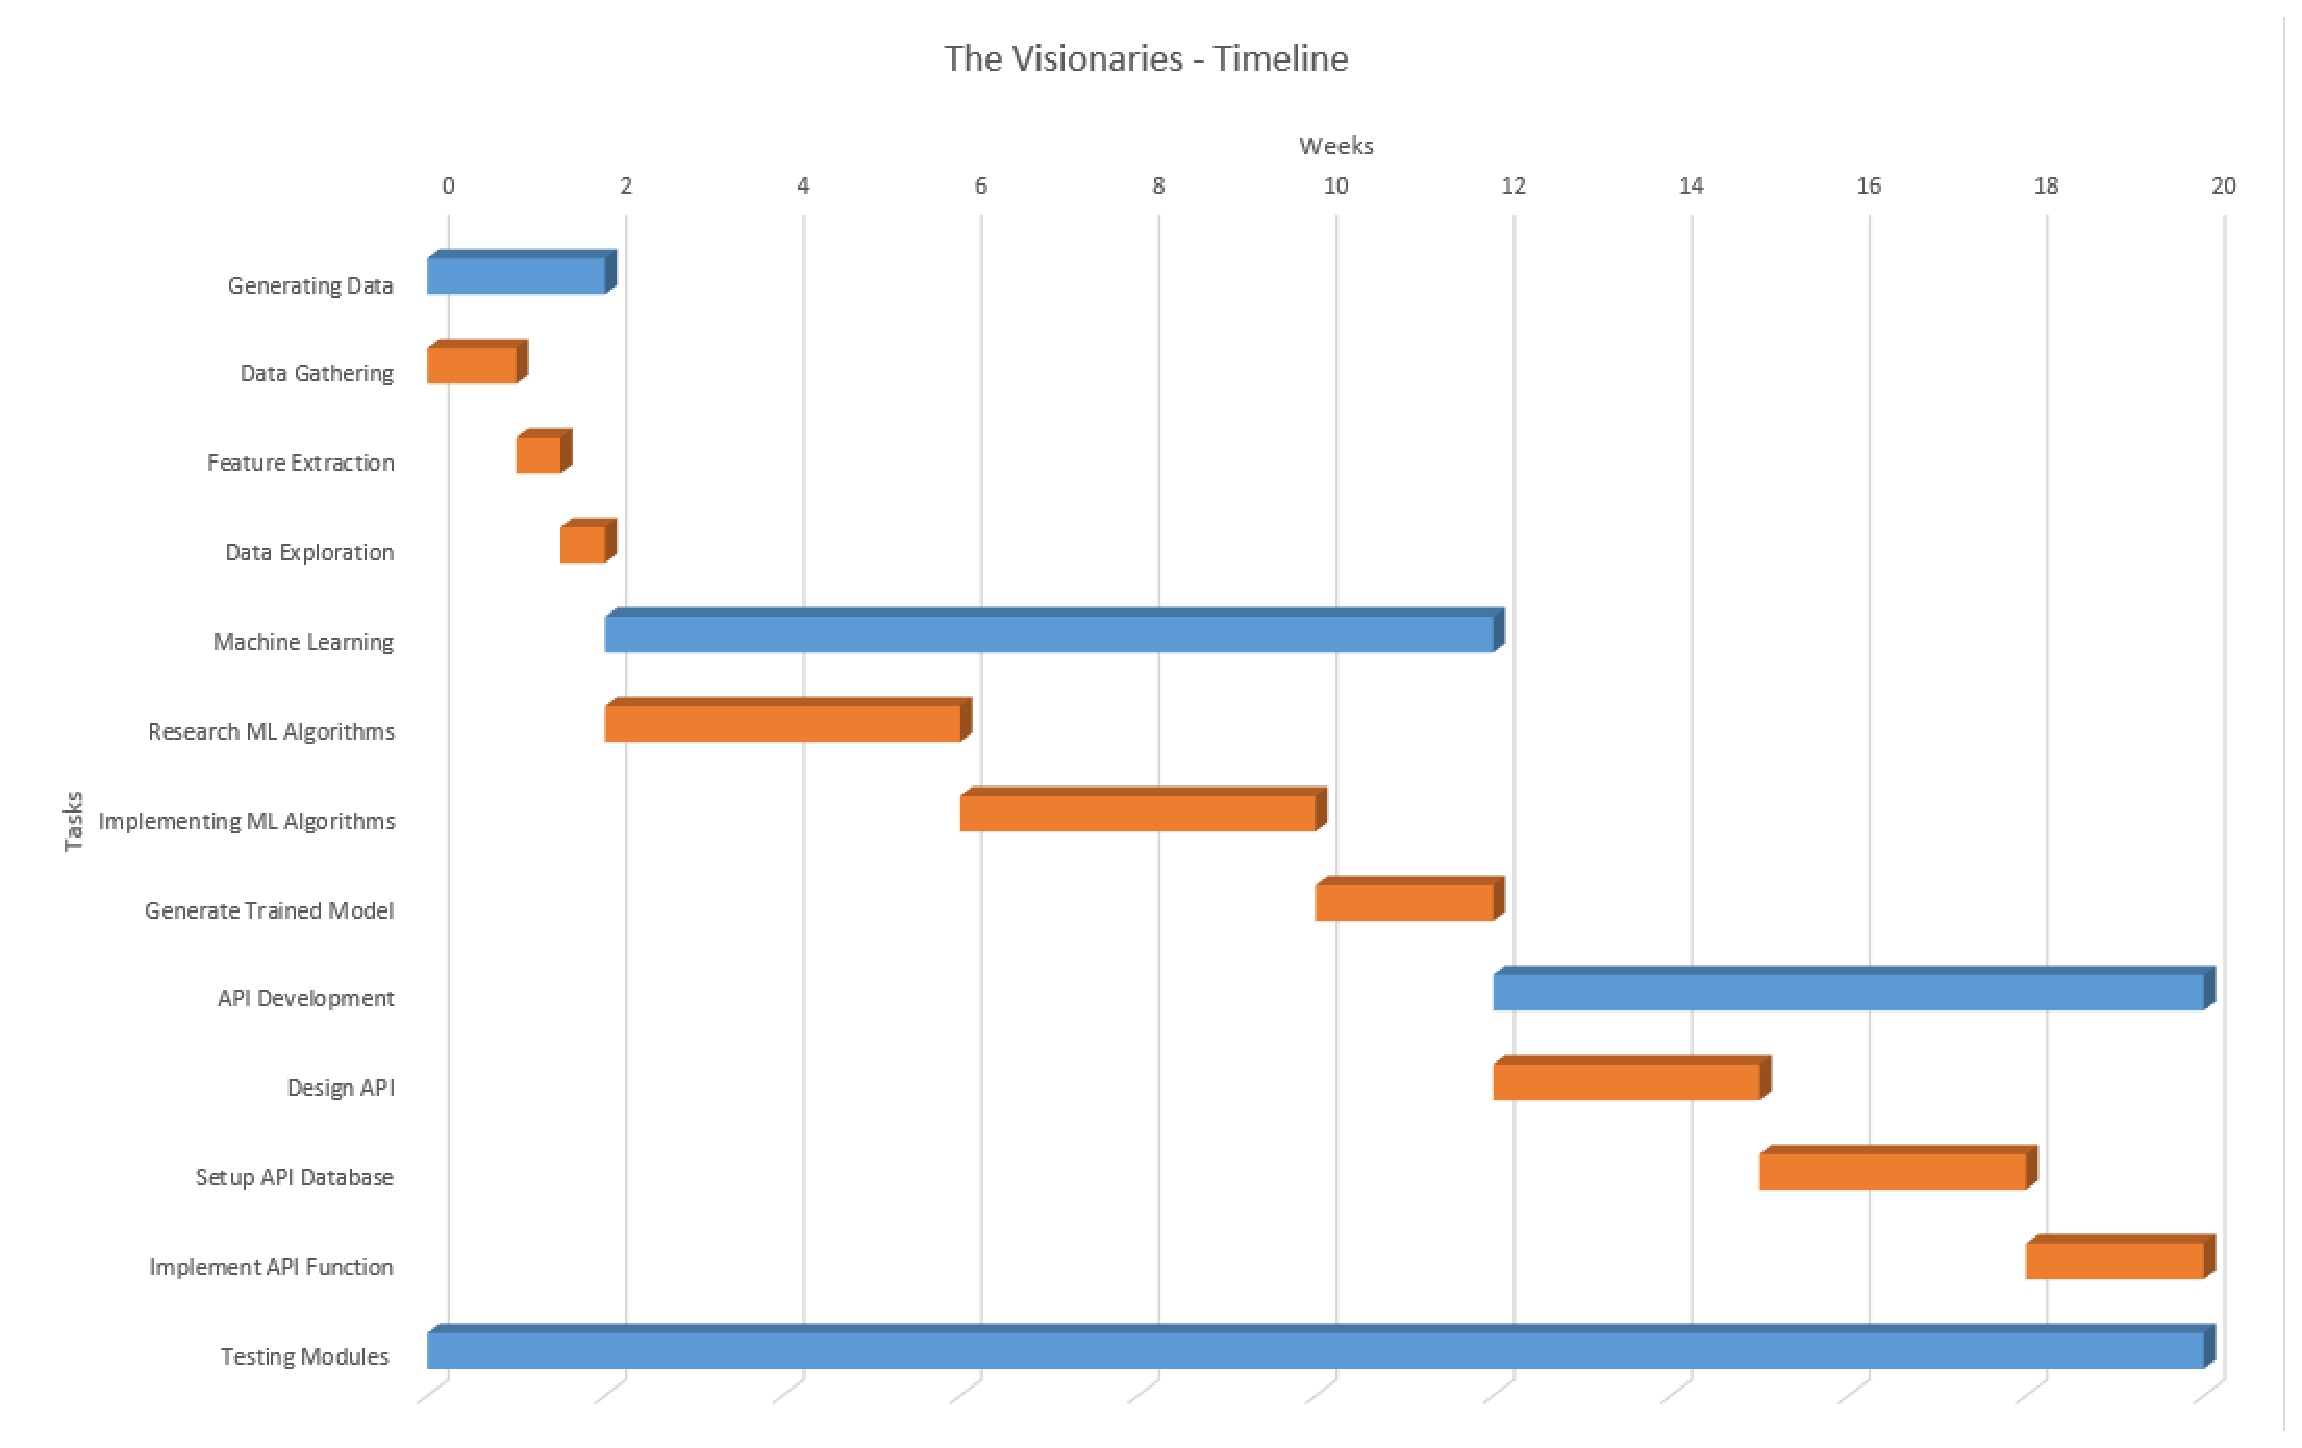
\includegraphics[height=10cm, width=17cm]{Timeline.eps}
        \caption{Gantt Chart of Project Dependencies}
        \label{fig:timeline}
    \end{figure}

The table below shows a more detailed explanation of their timeline graph. Each task has a start week as well as the duration it will take to complete:
\begin{center}
\captionof{table}{\textbf{Project Timeline Table}} \label{tab:title}
    \begin{tabular}{ |c|c|c| }
        \hline
        Tasks & Start Week & Duration (Weeks)\\ 
        \hline
        \textbf{Generating Data} & 0 & 20  \\ 
        \hspace{3mm}Data Gathering & 0 & 5 \\ 
        \hspace{3mm}Feature Extraction & 5 & 12 \\ 
        \hspace{3mm}Data Exploration & 5 & 15 \\
        \hline
        \textbf{Machine Learning Development} & 17 & 6 \\
        \hspace{3mm}Research ML Algorithms & 17 & 3 \\
        \hspace{3mm}Implementing ML Algorithm & 17 & 3 \\ 
        \hspace{3mm}Generate Trained Model & 18 & 5 \\
        \hline
        \textbf{API Development} & 18 & 2 \\
        \hspace{3mm}Design API & 18 & 1 \\
        \hspace{3mm}Setup API Database & 18 & 1 \\ 
        \hspace{3mm}Implementing API Function & 18 & 2 \\
        \hline
        \textbf{Testing Modules} & 0 & 25 \\
        \hline
    \end{tabular}
\end{center}
\section{Conclusion}
\begin{singlespace}
The end result of C3V will be an API that can return a predicted number of emergency calls of a given type for a given year and location within Levrum's target city of Charlotte, NC. 
The team will document the results of various analyses that was performed on the data, and show which of the analyses and features produce the result with the highest predictive power.
In addition, the team will provide Levrum with a set of tools to automate the majority of the process the team used to retrieve, consolidate, and transform the data necessary to make the same predictions for other cities.

\end{singlespace}

% REFERENCES
\newpage    
\bibliography{DesignDocRef}{}
\bibliographystyle{ieeetr}
\end{singlespace}
\end{document}
